\documentclass[11pt,a4paper]{article}
\usepackage[dvipsnames]{xcolor}
\usepackage[T1]{fontenc}
\newcommand{\hsh}[1]{{\texttt{\scriptsize #1}}}
\usepackage[utf8]{inputenc}
\usepackage{lmodern,microtype}
\usepackage{amsmath,amssymb,booktabs,graphicx,array,caption,url}
\usepackage[a4paper,margin=2.3cm]{geometry}
\usepackage[colorlinks=true,linkcolor=blue!50!black,urlcolor=blue!50!black,citecolor=blue!50!black]{hyperref}
\captionsetup{font=small,labelfont=bf}
\setlength{\parindent}{0pt}\setlength{\parskip}{4pt}

\usepackage[italian]{babel}
\title{\textbf{med6m: un adattatore LoRA per Qwen3-8B sul QA medico a scelta multipla}\\[2pt]\large Evidenza su test sigillato per il checkpoint 443 a scala LoRA 0.5}
\author{Giovanni Del Papa --- ricercatore indipendente, Italia\\ \small Progetto \emph{Lo Scienziato Dilettante GDP}}
\date{2 novembre 2026\\ \small Versione 1.0 --- DOI \href{https://doi.org/10.5281/zenodo.23895100}{10.5281/zenodo.23895100}\\ \small Hugging Face \texttt{odelpa/qwen3-8b-med6m} $\cdot$ GitHub \texttt{usergdp136/qwen3-8b-med6m}}
\begin{document}\maketitle
\begin{abstract}
Rilasciamo un adattatore LoRA (rango 64) per \texttt{unsloth/Qwen3-8B-unsloth-bnb-4bit}, addestrato con QLoRA su un mix medico di sei mesi (MedMCQA-train, MedQA-train, Wikipedia medica italiana e inglese) con il 22\% di replay generale. Su un test \emph{sigillato e a uso singolo} di 3\,766 item medici a scelta multipla (MedMCQA, MedQA, sei sottodomini medici di MMLU, PubMedQA) l'adattatore a scala LoRA $s=0.5$ migliora l'accuratezza rispetto al modello base di $+2.34$ punti percentuali (pp), IC 95\% bootstrap appaiato $[+1.14,+3.53]$, McNemar esatto $p=1.4\times10^{-4}$ (306 item corretti solo con l'adattatore contro 218 solo con la base). Il guadagno si concentra su MedMCQA ($+2.89$ pp) e PubMedQA ($+2.78$ pp); MedQA e MMLU-med sono positivi ma con IC che includono lo zero; la guardia generale italiana (ARC-it) non mostra regressioni ($+0.74$ pp, IC $[-1.29,+2.76]$). Limiti importanti: l'artefatto valutato è il checkpoint 443, non il finale 886; la valutazione usa la log-probabilità della lettera di risposta, non la generazione libera; non si afferma alcuna validità clinica.
\end{abstract}

\section{Metodo}
\paragraph{Modello e adattatore.} Base: Qwen3-8B (Apache-2.0), caricato a 4 bit NF4 (bitsandbytes). L'adattatore è una LoRA su tutte le proiezioni di attenzione e MLP (\texttt{q,k,v,o,gate,up,down}), rango $r=64$, $\alpha=64$, senza dropout. Per un peso congelato $W_0$ il peso adattato è
\begin{equation}\label{eq:lora}
W \;=\; W_0 \;+\; s\,\frac{\alpha}{r}\,B A,\qquad A\in\mathbb{R}^{r\times d_{\mathrm{in}}},\; B\in\mathbb{R}^{d_{\mathrm{out}}\times r},
\end{equation}
dove $s$ è la scala LoRA scelta in inferenza (qui $s=0.5$, $\alpha/r=1$): l'aggiornamento appreso viene applicato a metà intensità.

\paragraph{Addestramento.} Due stadi QLoRA consecutivi su una Tesla T4: lo stadio \texttt{S1\_v2} (885 passi, lr $5\times10^{-5}$, seed 3407) sulle sole quattro fonti mediche; lo stadio \texttt{S1\_v2r} (886 passi pianificati, lr $1.3\times10^{-5}$, warm-up 25, seed 3408, accumulo gradienti 16, lunghezza massima 2048), inizializzato dall'ultimo adattatore dello stadio 1 e con il 22\% di replay (OASST2, Aya, Dolly, Wikipedia italiana, FineWeb-Edu, FineWeb-2-it) per limitare l'oblio. \textbf{L'artefatto pubblicato è il checkpoint 443 dello stadio \texttt{S1\_v2r}} (50\% dello stadio). Per il secondo stadio erano pianificati circa $29.5$ M di token target efficaci (medico 78\%, replay 22\%).

\section{Protocollo di valutazione}
Ogni item è valutato con la log-probabilità della lettera di risposta. Con il chat template (thinking disattivato) e il prompt troncato a 2048 token, la predizione è
\begin{equation}\label{eq:mc}
\hat y \;=\; \arg\max_{\ell\in\mathcal{L}} \; z_\ell ,
\end{equation}
dove $z_\ell$ è il logit del token successivo per la lettera $\ell$ (con e senza spazio iniziale) e $\mathcal{L}$ l'insieme delle lettere delle opzioni. La generazione libera \emph{non} è valutata. Benchmark: MedMCQA (validation), MedQA-USMLE-4-options (test), sei sottodomini medici di MMLU, PubMedQA (\texttt{pqa\_labeled}, solo domanda, senza contesto) e ARC-Italian (challenge) come guardia generale. La divisione dev/test è deterministica: SHA-1 di \texttt{"split|"+ID}, parità del digest. I dati di training sono stati decontaminati rispetto a dev e test con corrispondenza di 10-grammi. Il test sigillato è stato eseguito \emph{una sola volta} (marcatore \texttt{TEST\_USED}, 1 novembre 2026) per la base e per il checkpoint 443 a $s\in\{0.5,0.75\}$; il test è quindi consumato e non può essere riusato per altre selezioni.

\section{Statistica}
Per l'item $i$ siano $b_i,c_i\in\{0,1\}$ la correttezza di base e adattatore e $d_i=c_i-b_i\in\{-1,0,1\}$. L'effetto riportato è
\begin{equation}\label{eq:delta}
\Delta_{\mathrm{pp}} \;=\; \frac{100}{n}\sum_{i=1}^{n} d_i \;=\; \frac{100\,(n_{+}-n_{-})}{n},
\end{equation}
con $n_+$ ($n_-$) gli item corretti solo con l'adattatore (solo con la base). Gli intervalli di confidenza sono bootstrap percentile appaiati, implementati come ricampionamento multinomiale dei conteggi,
\begin{equation}\label{eq:boot}
\begin{gathered}
(n_-^*,n_0^*,n_+^*)\sim\mathrm{Mult}\!\big(n;\,\hat p\big),\quad \hat p=\big(\tfrac{n_-}{n},\tfrac{n_0}{n},\tfrac{n_+}{n}\big)\\[3pt] \mathrm{IC}_{95}=\big[q_{0.025},\,q_{0.975}\big]\big\{100\,\tfrac{n_+^*-n_-^*}{n}\big\},
\end{gathered}\end{equation}
con $B=20\,000$ repliche e seed 20261101. Il test di McNemar esatto bilaterale sulle coppie discordanti ($n_-+n_+=m$) è
\begin{equation}\label{eq:mcn}
p \;=\; \min\Big\{1,\; 2\sum_{k=0}^{\min(n_-,n_+)}\binom{m}{k}2^{-m}\Big\}.
\end{equation}
Il pool concatena i quattro benchmark medici e pesa gli \emph{item}, non i benchmark. Non è applicata alcuna correzione per confronti multipli; i valori $p$ per benchmark sono descrittivi.

\section{Risultati sul test sigillato}
La Tabella~\ref{tab:main} riporta il risultato primario (scala 0.5); la Figura~\ref{fig:forest} mostra le differenze con gli IC per entrambe le scale; la Figura~\ref{fig:acc} le accuratezze e la Figura~\ref{fig:disc} guadagni e perdite per item.
\begin{table}[h]\centering\small
\caption{Test sigillato, checkpoint 443, \textbf{scala 0.5} contro la base. Accuratezza in \%; ``+/$-$'' = item corretti solo con l'adattatore / solo con la base. $\Delta$ in punti percentuali con IC 95\% bootstrap; $p$ McNemar esatto.}\label{tab:main}
\begin{tabular}{lrrrrcrr}\toprule
Set & $n$ & Base & Adattatore & $\Delta$ (pp) & IC 95\% & +/$-$ & McNemar $p$ \\ \midrule
MedMCQA & 2078 & 57.31 & 60.20 & +2.89 & [+1.15, +4.62] & 200/140 & 0.001 \\
MedQA & 646 & 62.85 & 64.40 & +1.55 & [$-$1.55, +4.64] & 57/47 & 0.378 \\
MMLU-med & 538 & 78.25 & 79.00 & +0.74 & [$-$1.67, +3.16] & 25/21 & 0.659 \\
PubMedQA & 504 & 57.94 & 60.71 & +2.78 & [+0.60, +5.16] & 24/10 & 0.024 \\
\midrule
Pool medico (n=3766) & 3766 & 61.34 & 63.67 & +2.34 & [+1.14, +3.53] & 306/218 & $<$0.001 \\
\midrule
ARC-it (guardia) & 543 & 88.21 & 88.95 & +0.74 & [$-$1.29, +2.76] & 17/13 & 0.585 \\
\bottomrule\end{tabular}\end{table}

\begin{table}[h]\centering\small
\caption{Stesso test, scala 0.75 (riportata per trasparenza; entrambe le scale sono state valutate sullo stesso test consumato).}\label{tab:s075}
\begin{tabular}{lrrrrcrr}\toprule
Set & $n$ & Base & Adattatore & $\Delta$ (pp) & IC 95\% & +/$-$ & McNemar $p$ \\ \midrule
MedMCQA & 2078 & 57.31 & 60.97 & +3.66 & [+1.83, +5.49] & 230/154 & $<$0.001 \\
MedQA & 646 & 62.85 & 63.31 & +0.46 & [$-$2.63, +3.72] & 56/53 & 0.848 \\
MMLU-med & 538 & 78.25 & 79.00 & +0.74 & [$-$1.86, +3.35] & 28/24 & 0.678 \\
PubMedQA & 504 & 57.94 & 59.72 & +1.79 & [$-$0.40, +4.17] & 22/13 & 0.175 \\
\midrule
Pool medico (n=3766) & 3766 & 61.34 & 63.78 & +2.44 & [+1.17, +3.69] & 336/244 & $<$0.001 \\
\midrule
ARC-it (guardia) & 543 & 88.21 & 88.77 & +0.55 & [$-$1.66, +2.76] & 20/17 & 0.743 \\
\bottomrule\end{tabular}\end{table}

\begin{figure}[h]\centering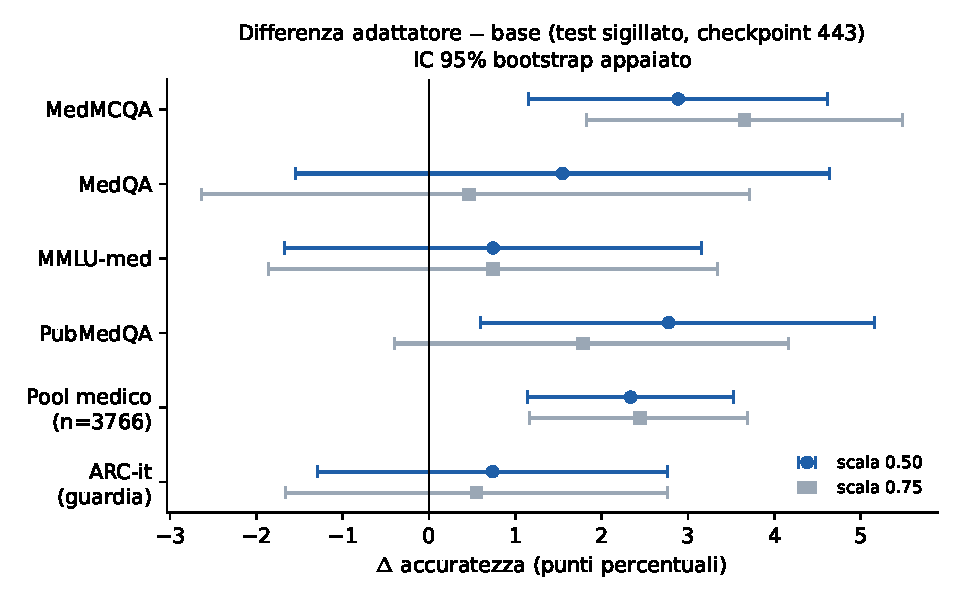
\includegraphics[width=.82\linewidth]{../figures/fig1_forest_it.pdf}\caption{Adattatore meno base, test sigillato. Punti: $\Delta_{\mathrm{pp}}$ (Eq.~\ref{eq:delta}); barre: IC 95\% (Eq.~\ref{eq:boot}).}\label{fig:forest}\end{figure}
\begin{figure}[h]\centering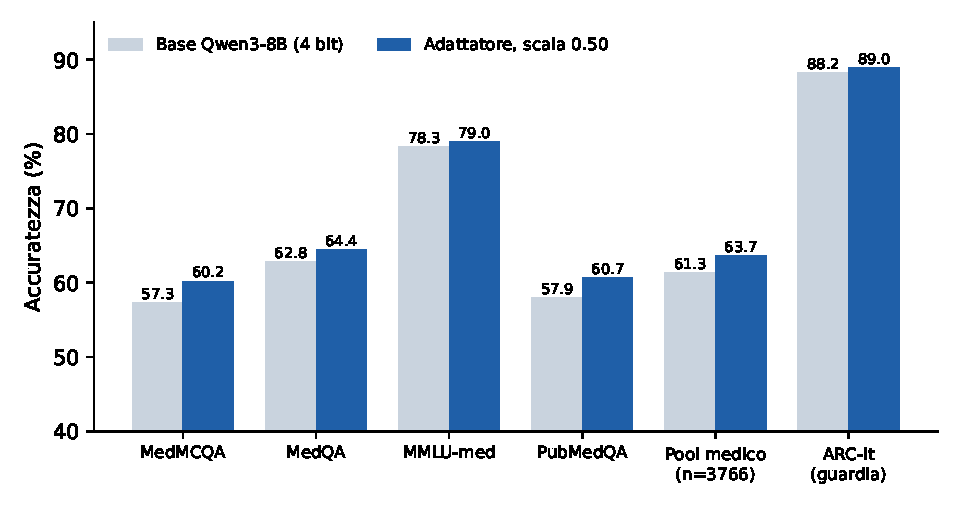
\includegraphics[width=.82\linewidth]{../figures/fig2_acc_it.pdf}\caption{Accuratezza di base e adattatore (scala 0.5).}\label{fig:acc}\end{figure}
\begin{figure}[h]\centering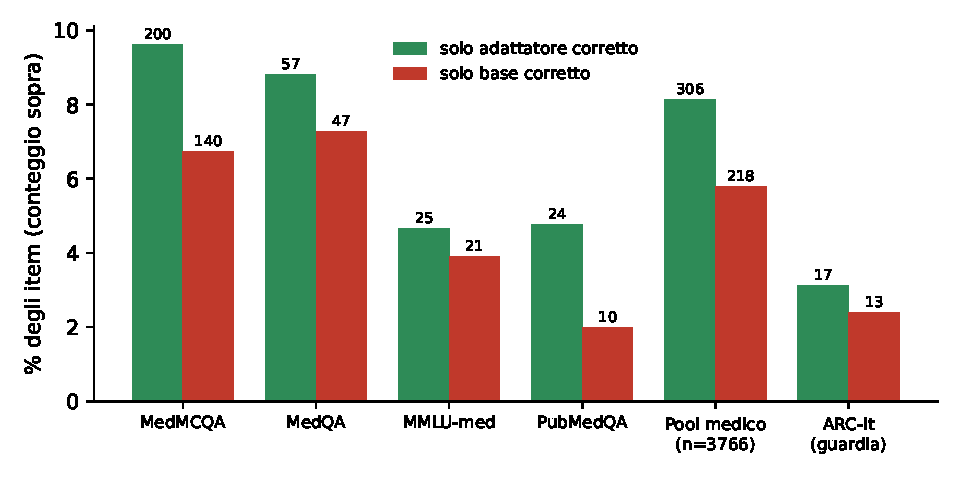
\includegraphics[width=.82\linewidth]{../figures/fig3_disc_it.pdf}\caption{Item corretti solo con l'adattatore ($n_+$) contro solo con la base ($n_-$).}\label{fig:disc}\end{figure}

\paragraph{Lettura.} Il pool medico migliora di $+2.34$ pp (l'IC esclude lo 0, $p=1.4\times10^{-4}$). Il risultato è guidato da due benchmark: MedMCQA (il mix di training contiene MedMCQA-train, quindi parte del guadagno è adattamento in-distribution al formato d'esame) e PubMedQA. MedQA ($+1.55$) e MMLU-med ($+0.74$) hanno IC che includono lo zero: \emph{non} sono miglioramenti confermati. La guardia ARC-it non mostra regressioni sul test sigillato. Le scale 0.5 e 0.75 sono statisticamente indistinguibili sul pool ($+2.34$ contro $+2.44$ pp).

\section{Checkpoint finale 886 sul dev (non indipendente)}
Il checkpoint finale è stato valutato solo sullo split dev, che ha guidato le decisioni di training (gate, scala). Non è quindi una conferma indipendente e non è l'artefatto pubblicato.
\begin{table}[h]\centering\small
\caption{Split DEV, checkpoint finale 886 a scala 1.0 contro la base (pool $n=3779$).}
\begin{tabular}{lrrrrcr}\toprule Set & $n$ & Base & Finale & $\Delta$ (pp) & IC 95\% & +/$-$ \\ \midrule
MedMCQA & 2105 & 56.25 & 59.48 & +3.23 & [+1.38, +5.08] & 238/170 \\
MedQA & 627 & 62.04 & 65.87 & +3.83 & [+0.48, +7.18] & 70/46 \\
MMLU-med & 551 & 77.13 & 76.41 & $-$0.73 & [$-$3.63, +2.18] & 30/34 \\
PubMedQA & 496 & 53.83 & 55.44 & +1.61 & [$-$0.81, +4.23] & 25/17 \\
Pool medico  & 3779 & 59.94 & 62.48 & +2.54 & [+1.22, +3.84] & 363/267 \\
ARC-it (guardia) & 589 & 86.42 & 84.55 & $-$1.87 & [$-$4.07, +0.34] & 18/29 \\
\bottomrule\end{tabular}\end{table}
\begin{figure}[h]\centering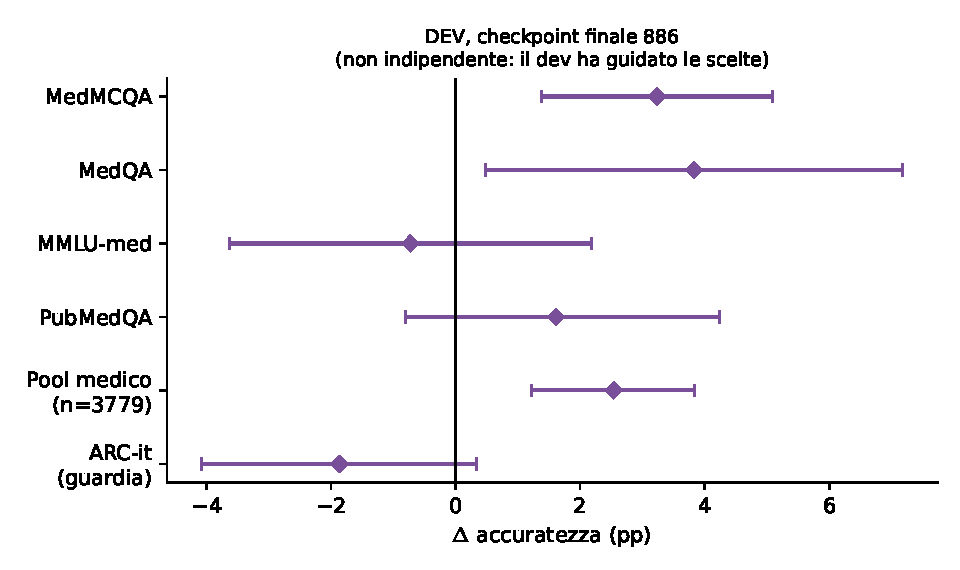
\includegraphics[width=.78\linewidth]{../figures/fig4_dev886_it.pdf}\caption{Differenze sul dev per il checkpoint finale 886.}\end{figure}
Sul dev il finale guadagna $+2.54$ pp sul pool medico ma perde $-0.73$ pp su MMLU-med e $-1.87$ pp su ARC-it (IC che includono 0). Il gate storico (due errori standard) lo ammetteva; un criterio più severo (margine $-0.5$ pp, soglia ARC-it 85.42\%) lo respingerebbe. Il criterio del gate è stato rivisto il 31 ottobre 2026 e il checkpoint al 50\% è stato rivalutato post hoc. Per questi motivi pubblichiamo il checkpoint 443 (testato sul set sigillato) e \emph{non} il finale.

\section{Limiti e rischi}
\begin{itemize}
\item \textbf{Checkpoint contro finale.} L'evidenza riguarda il checkpoint 443; nulla è affermato per l'886.
\item \textbf{Post-selezione.} Due scale sono state valutate sullo stesso test consumato; la scala 0.5 è stata preferita su criteri dev (variazione ARC-it minore, guadagno PubMedQA maggiore), ma non esiste una scelta preregistrata.
\item \textbf{Nessuna correzione per molteplicità}; gli IC per benchmark sono descrittivi. MedQA e MMLU-med non sono significativi.
\item \textbf{Tipo di compito.} Solo log-probabilità della lettera a scelta multipla; nessuna risposta libera, nessuna valutazione di sicurezza, nessuna validazione clinica. \emph{Non usare per consigli medici.}
\item \textbf{Controlli di capacità generale in sospeso:} GSM8K e IFEval sul checkpoint 443 \emph{non} sono ancora stati eseguiti; è riportata solo la guardia ARC italiana.
\item \textbf{Provenienza.} MedMCQA-train è dichiarato Apache-2.0 ma la provenienza delle domande d'esame non è verificata in modo indipendente; le revisioni di modello/dataset non erano fissate al momento dell'addestramento (riportiamo le revisioni in cache sulla macchina di training, Appendice~A).
\item \textbf{Audit di rete.} Una revisione statica del codice di training/valutazione non ha trovato endpoint diversi da Hugging Face e ha \texttt{report\_to='none'}; un audit dinamico (traffico) non è stato eseguito retroattivamente (Appendice~B).
\end{itemize}

\section{Licenze e attribuzione}
Modello base: Qwen3-8B, Apache-2.0 (\copyright{} Qwen Team / Alibaba Cloud; ripacchettamento a 4 bit di Unsloth). Fonti di training e licenze: MedMCQA-train (Apache-2.0, dichiarata), MedQA-train (MIT, split train di \texttt{openlifescienceai/medqa}), Wikipedia IT/EN (CC BY-SA 3.0 / GFDL), Dolly-15k (CC BY-SA 3.0), OASST2 e Aya (Apache-2.0), FineWeb-Edu e FineWeb-2 (ODC-By 1.0). Tutte permettono l'uso commerciale; nessuna è non commerciale. Poiché diverse fonti sono share-alike, adattatore, articolo e figure sono rilasciati con licenza \textbf{CC BY-SA 4.0} e il codice con Apache-2.0; l'attribuzione è in \texttt{ATTRIBUTION.md}. Se la clausola share-alike si estenda giuridicamente ai pesi del modello è questione non risolta; la applichiamo in via cautelativa.

\section{Riproducibilità}
\texttt{code/recompute.py} ricalcola ogni numero delle tabelle dai conteggi appaiati (CPU, NumPy, senza rete); \texttt{code/make\_figures.py} rigenera le figure. L'audit assistito da Codex e il nostro ricalcolo concordano alla seconda cifra decimale (pool $+2.3367$, IC $[1.1418,3.5316]$). Gli script di training e valutazione sono forniti per ispezione; richiedono l'ambiente originale (Unsloth 2026.10.7, Transformers 5.17.0, PEFT 0.21.2, TRL 1.15.0, bitsandbytes 0.50.2, PyTorch 2.11.0+cu128).

\sloppy
\appendix
\section{Artefatti fissati}
\begin{table}[h]\centering\footnotesize
\begin{tabular}{p{5.6cm}p{9.9cm}}\toprule Artefatto & SHA-256 / revisione \\ \midrule
\hsh{adapter\_model.safetensors} & \hsh{0dfdebe51f325a0d0e1cc5851193a03c4d6aef898ba3b3a595145ab508c4a5bf} \\
\texttt{adapter\_config.json} & \hsh{dcabc2e1d6661d1ad5a18f475a7fd08c875e8cba8664ffbea95bff32d0ce6943} \\
\texttt{tokenizer.json} & \hsh{476870a1f2fb6f6a2759a6ede2383bf9d5d738f17844563b65c91965b722ae09} \\
Base \hsh{unsloth/Qwen3-8B-unsloth-bnb-4bit} & revision \hsh{62efd7f9d748e394734a7adae2adf96e13a2abc8} (in cache dal 24 ott 2026) \\
\texttt{openlifescienceai/medmcqa} & \hsh{91c6572c454088bf71b679ad90aa8dffcd0d5868} \\
\texttt{GBaker/MedQA-USMLE-4-options} & \hsh{0fb93dd23a7339b6dcd27e241cb9b5eca62d4d18} \\
\texttt{cais/mmlu} & \hsh{c30699e8356da336a370243923dbaf21066bb9fe} \\
\texttt{qiaojin/PubMedQA} & \hsh{9001f2853fb87cab8d220904e0de81ac6973b318} \\
\texttt{sapienzanlp/arc\_italian} & \hsh{1860d09fba59b9b2576335ab472346f63c1becc8} \\
\texttt{wikimedia/wikipedia} & \hsh{b04c8d1ceb2f5cd4588862100d08de323dccfbaa} \\
\bottomrule\end{tabular}\end{table}
\section{Nota sull'audit di rete}
Ambito: il codice med6m (\texttt{build\_s1v2r.py}, \texttt{train\_stage\_r.py}, \texttt{eval\_mc.py}, \texttt{s0\_data.py}, \texttt{s0b\_data.py}). Esito: l'accesso di rete è limitato ai download di dataset/hub Hugging Face per la preparazione dei dati; \texttt{report\_to='none'} (nessun W\&B o altro tracker); training e scoring leggono file JSONL locali. \texttt{pmc.py} (Europe PMC S3) appartiene agli helper di preparazione dati e non fa parte di training/valutazione. Non verificato: nei launcher non sono stati trovati flag d'ambiente (\texttt{HF\_HUB\_OFFLINE}, \texttt{UNSLOTH\_DISABLE\_STATISTICS}), quindi la telemetria delle librerie non può essere esclusa; si raccomanda una riesecuzione offline pulita con cattura del traffico.
\begin{thebibliography}{9}
\bibitem{qlora} T.~Dettmers et al., \emph{QLoRA: Efficient Finetuning of Quantized LLMs}, 2023. \url{https://arxiv.org/abs/2305.14314}
\bibitem{lora} E.~Hu et al., \emph{LoRA: Low-Rank Adaptation of Large Language Models}, 2021. \url{https://arxiv.org/abs/2106.09685}
\bibitem{qwen3} Qwen Team, \emph{Qwen3 Technical Report}, 2025. \url{https://arxiv.org/abs/2505.09388}
\bibitem{medmcqa} A.~Pal et al., \emph{MedMCQA}, CHIL 2022. \url{https://arxiv.org/abs/2203.14371}
\bibitem{medqa} D.~Jin et al., \emph{What disease does this patient have? (MedQA)}, 2020. \url{https://arxiv.org/abs/2009.13081}
\bibitem{pubmedqa} Q.~Jin et al., \emph{PubMedQA}, EMNLP 2019. \url{https://arxiv.org/abs/1909.06146}
\bibitem{mmlu} D.~Hendrycks et al., \emph{Measuring Massive Multitask Language Understanding}, ICLR 2021. \url{https://arxiv.org/abs/2009.03300}
\end{thebibliography}
\end{document}
